\documentclass[../../note.tex]{subfiles}
%\newcommand\SZQ[1]{{\color{blue}\footnotesize\sffamily [SZQ: #1]}}
\begin{document}

\chapter{Functional Analysis}
\section{Metric Space}
\begin{definition}[Metrix Spaces]
    Define set $X$. Define a metric: $d: X \times X \rightarrow [0, \infty)$ 
    \begin{itemize}
        \item $d(x, y) = 0 \Longleftrightarrow x = y$
        \item $d(x, y) = d(y,x)$
        \item $d(x,y) \leq d(x,z) + d(z,y)$ (triangle inequality)
    \end{itemize}
\end{definition}

Summary: $X$ set + $d: X \times X \rightarrow [0,\infty)$ metric = metric space $(X, d)$.
\begin{example}
    \begin{itemize}
        \item $X = \mathbb{C}, d(x,y) = \vert x-y \vert$
        \item $X = \mathbb{R}^n, d(x,y) = \sqrt{(x_1 - y_1)^2 +(x_2 - y_2)^2 +\dots+(x_n - y_n)^2 }$ (Euclidean metric)
        \item $X = \mathbb{R}^n, d(x,y) = \max\left\{\vert x_1 - y_1 \vert,..., \vert x_n - y_n \vert \right\}$. It is possible that $d(x,y) = d(x,z)$.
        \item $X$ any set ($\neq \emptyset$), we define
        \begin{align}
            d(x,y)
            &= \left\{ \begin{matrix}
                0,& x = y \\
                1,& x \neq y
            \end{matrix}\right.
        \end{align}
        Now, let's check whether this is a metrix space. Conditions (1) and (2) are verified easily. We focus on the verification of (3): choose $x,y,z \in X$. 
        
        For the first case: $x = y$: $d(x,y) = 0 \leq d(x,z) + d(z,y)$.

        For the second case: $x \neq y$: $d(x,y) = 1 \leq \left\{d(x,z)~or~d(z,y)\right\} = d(x,z) + d(z,y)$.

        This is called \textbf{discrete matric}.
    \end{itemize}
\end{example}

\section{Open and Closed Sets}
\begin{definition}[Open Ball]
    $(X,d)$ a metrix space. Define 
    \begin{align}
        B_{\epsilon}(x)
        &:= \left\{y \in X \vert d(x,y) < \epsilon \right\},
    \end{align}
    whihc is called the open ball of radiue $\epsilon > 0$ centered at $x$.
\end{definition}

\begin{definition}[Open Sets]
    $A \subseteq X$ is called open is for each $x \in A$ there is an open ball with $B_{\epsilon}(x) \subseteq A$.
\end{definition}
We have nice pic for this.

\begin{definition}[Boundary Points]
    $A \subseteq X$, $x \in X$ is called a boundary point for $A$ if for all $\epsilon > 0$: $B_{\epsilon}(x) \cap A = \emptyset$ and  $B_{\epsilon}(x) \cap A^c = \emptyset$. [$A^c:= X \backslash A$]

    Notation: $\partial A: \left\{x \in X \vert x~is~boundary~point~for~A \right\}$
\end{definition}
We have nice pic for this.

Remember: $A$ open $\Longleftrightarrow$ $A \cap \partial A = \emptyset$.

\begin{definition}[Closed Sets]
    $A \subseteq X$ is called closed if $A^c:= X \backslash A$ is open.
\end{definition}

\begin{definition}[Closure]
    $\overline{A}:= A \cup \partial A$ (always closed!)
\end{definition}

\begin{example}
    $X:= (1,3] \cup (4, \infty), d(x,y):= \vert x - y \vert, (X,d)$ is a metrix space.
    \begin{itemize}
        \item $A:= (1,3] \subseteq X$ open? 
        
        For $x \in A, x \neq 3$, define $\epsilon:= \frac{1}{2}\min\left(\vert 1-x \vert, \vert 3 - x \vert \right)$. Then $B_{\epsilon}(x) \subseteq A$.

        For $x = 3$: $B_1(x) = \left\{y \in X \vert d(x,y) <1 \right\} = (2,3] \subseteq A$.
        \item A is also closed!
        \item $C:= (1,2]$, $\partial C = \left\{2\right\}$, $\overline{C} = C$.
    \end{itemize}
\end{example}

\section{Sequence, Limits and Closed Sets}
\begin{definition}[Sequence]
    Sequence in $X$: $x_1,x_2,\dots$ or $(x_n)_{n \in \mathbb{N}}$ or map $x: \mathbb{N} \rightarrow X$ / $n \mapsto x_n$.
\end{definition}

\begin{definition}[Convergence]
    A sequence $(x_n)_{n \in \mathbb{N}}$ in a metrix space $(X,d)$ is called convergence if there is $\tilde{x} \in X$ with $\forall \varepsilon \geq 0, \exists N \in \mathbb{N}, \forall n \geq N: d(x_n, \tilde{x}) < {\varepsilon}$. We write: $X_n \stackrel{n \rightarrow \infty}{\longrightarrow} \tilde{x}$ or $\lim_{n \rightarrow} x_n = \tilde{x}$.
\end{definition}

\begin{proposition}[Closed Sets]
    $A \subseteq X$ is closed $\Longleftrightarrow$ For every convergent sequence $(a_n)_{n \in \mathbb{N}} \subseteq A$, one has $\lim_{n \rightarrow \infty} a_n \in A$.
\end{proposition}
\begin{proof}
    ($\Longleftarrow$): Show it by contraposition! Assume $A$ is not closed.
    \begin{align}
        &\Longrightarrow A^c:= X \backslash A~\textrm{is not open.} \\
        &\Longrightarrow \textrm{There is an}~\tilde{x} \in A^c~\textrm{with}~B_{\varepsilon}(\tilde{x}) \cap A \neq \emptyset, \forall \varepsilon >0. \\
        &\Longrightarrow \textrm{There is a sequence}~(a_n)_{n \in \mathbb{N}}~with~a_n \in B_{1/n}(\tilde{x}) \cap A \\
        &\Longrightarrow \lim_{n \rightarrow \infty} a_n = \tilde{x} \neq A.
    \end{align}
    ($\Longrightarrow$): Show it by contraposition! Assume there is $(a_n)_{n \in \mathbb{N}} \subseteq A$ with $\tilde{x}:= \lim_{n \rightarrow \infty} \notin A$.
    \begin{align}
        &\Longrightarrow B_{\varepsilon}(\tilde{x}) \neq \emptyset, \forall \varepsilon >0 \\
        &\Longrightarrow A^c~\textrm{is not open} \\
        &\Longrightarrow A~\textrm{is not closed}.
    \end{align}
\end{proof}
\SZQ{This proof use many contrapositions. It is nice to get familiar with how to use contrapositions to prove. It also needs to know the inverse of $\forall$.}

\section{Cauchy Sequence and complete metric spaces}
\begin{example}
    $X = (0,3)$ with $d(x,y) = \vert x-y \vert$.

    $(0,3)$ is closed:
    \begin{itemize}
        \item complement $\emptyset$ is open
        \item each convergent sequence $(x_n)_{n \in \mathbb{N}} \subseteq (0,3)$ (with limit $\tilde{x} \in X$) satisfies $\tilde{x} \in (0,3)$
    \end{itemize}

    What is about the sequence $(\frac{1}{n})_{n \in \mathbb{N}}$?
    \begin{itemize}
        \item sequence in $X$
        \item $d(x_n, x_m) \stackrel{n, m \rightarrow \infty}{\longrightarrow} 0$ 
        \item it does not converge 
        $\Longrightarrow$ $(X,d)$~\textrm{is not complete} 
    \end{itemize}
\end{example}

\begin{definition}[Cauchy Sequence and Complete]
    Let $(X,d)$ be a metrix space. A sequence $(x_n)_{n \in \mathbb{N}} \subseteq X$ is called Cauchy sequence if $\forall \varepsilon 0, \exists N \in \mathbb{N}, \forall n,m \geq N: d(x_n, x_m)<\varepsilon$. $(X,d)$ is called complete if all Cauchy sequences converge.
\end{definition}

\begin{example}
    \begin{itemize}
        \item $X = [0,3]$ with $d(x,y) = \vert x - y \vert$ is complete.
        \item $X = (0,3)$ with 
        \begin{align}
            \left\{\begin{matrix}
                1,& x\neq y \\
                0,& x= y
            \end{matrix}
            \right.
        \end{align}
        is complete.
    \end{itemize}
    \begin{proof}
        Let $(x_n)_{n \in \mathbb{N}} \subseteq X$ be a Cauchy sequence. Take $\varepsilon =1/2$. Then there is an $N \in \mathbb{N}$ such that for all $n,m \geq N$, we have $d(x_n, x_m) <\frac{1}{2}$. By definition,  $d(x_n, x_m) = 0$. Hence, $x_n = x_m$.
    \end{proof}
\end{example}

\section{Norms and Banach Spaces}
\begin{definition}[Norm]
    \label{def: norm}
    $\mathbb{F} \in \left\{\mathbb{R}, \mathbb{C}\right\}$. Let $X$ be a $\mathbb{F}$-vector space. A map $\vert \vert \cdot \vert \vert: X \rightarrow [0, \infty)$ is called norm if 
    \begin{itemize}
        \item $\vert \vert x \vert \vert = 0 \Longleftrightarrow x = 0$ (postitive definite) 
        \item $\vert \vert \lambda \cdot x \vert \vert = \vert \lambda \vert \vert x \vert \vert $ for all $\lambda \in \mathbb{F}$, $x \in X$ (absolutely homogeneous) 
        \item $\vert \vert x \vert \vert \leq \vert \vert x \vert \vert + \vert \vert y \vert \vert$ for all $x,y \in X$ (triangle inequality)
    \end{itemize}
\end{definition}

\begin{definition}[Normed Space]
    $(X, \vert \vert \cdot \vert \vert)$ is then called a normed space.
\end{definition}

\textbf{Normed space is a special case of metric space!}

\begin{lemma}[Relationship between normed space and metric space]
    If $\vert \vert \cdot \vert \vert$ is a norm for the $\mathbb{F}$-vector space $X$, then $d_{\vert \vert \cdot \vert \vert}(x,y):= \vert \vert x-y \vert \vert$ defines a metric for the set $X$.
\end{lemma}
\begin{proof}
    This can be proved by the defnition of norm.
\end{proof}

\begin{definition}[Banach space]
    If $(X, d_{\vert \vert \cdot \vert \vert})$ is a complete metric space, then the normed space $(X, \vert \vert \cdot \vert \vert)$ is called a Banach space.
\end{definition}

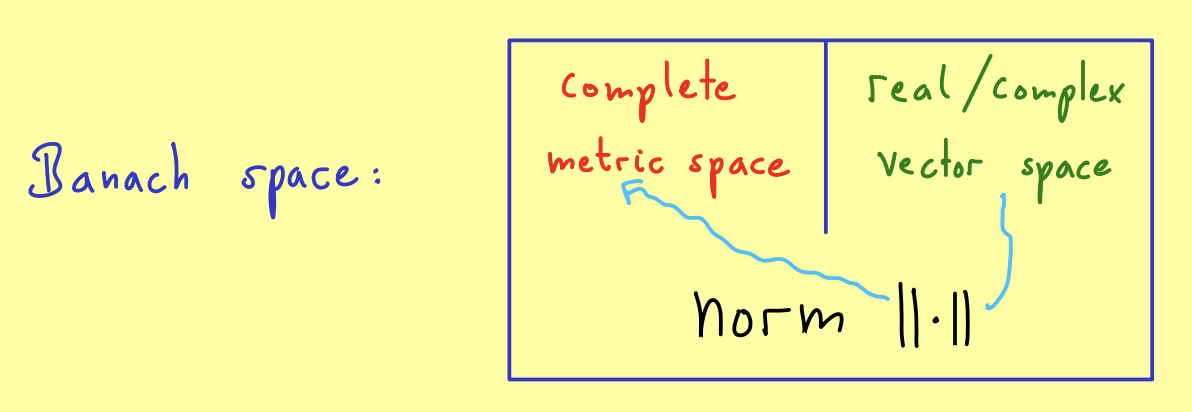
\includegraphics[scale = 0.6]{../figures/banach space.png}

The figure is very impressive and informative!


\section{Examples of Banach Spaces}





\section{Part 12: Continuity}
\begin{definition}[Continuity for metric spaces]
    $(X,d_Y)$, $(Y,d_Y)$ are two metric spaces. A map $f: X \rightarrow Y$ is called: 
    \begin{itemize}
        \item continuous if $f^{-1}[B]$ is open in $X$ for all open sets $B \subseteq Y$.
        \item sequentially continuous if for all $\tilde{x} \in X$ and $(x_n)_{n \in \mathbb{N}} \subseteq X$ with $x_n \stackrel{n \rightarrow \infty}{\longrightarrow} \tilde{x}$ holds $f(x_n) \stackrel{n \rightarrow \infty}{\longrightarrow} f(\tilde{x})$.
    \end{itemize}
\end{definition}
These are shown by figs.

\begin{lemma}
    For metrc spaces, continuous and sequentially continuous are equivalent. But for topological spaces, they are different.
\end{lemma}

\begin{example}
    \begin{itemize}
        \item $(X,d_X)$ discrete metric space, $(Y, d_Y)$ any metrix space $\Longrightarrow$ all $f: X \rightarrow Y$ are continuous.
        \item $(X,d_X)$, $(Y, d_Y)$ metric spaces, $Y_0 \in Y$ fixed. $\Longrightarrow$ $f: X \rightarrow Y$, $x \mapsto y_0$ is always continuous.
        \item $(X, \Vert \cdot \Vert)$ normed space, $Y = \mathbb{R}$ with standard metric. $\Longrightarrow$ $f: X \rightarrow \mathbb{R}$, $x \mapsto \Vert x \Vert$ is continuous.
        \begin{proof}
            Let $(x_n)_{n \in \mathbb{N}} \subseteq X$ sequence with limit $\tilde{x} \in X$. Then:
            \begin{align}
                f(x_n) 
                &= \Vert x_n \Vert \\
                &= \Vert x_n -\tilde{x} + \tilde{x} \Vert \\
                &\qquad\eqnote{By triangle inequality \ref{def: norm}} \nonumber \\
                &\leq \Vert x_n -\tilde{x} \Vert + \Vert \tilde{x}\Vert \\
                &= d(x_n, \tilde{x}) + f(\tilde{x}) \\
                &\Longrightarrow \lim{n \rightarrow \infty} f(x_n) \leq f(\tilde{x}).
            \end{align}
            We also hold:
            \begin{align}
                f(\tilde{x})
                &= \Vert \tilde{x} \Vert \\
                &= \Vert \tilde{x}-x_n + x_n \Vert \\
                &\qquad\eqnote{By triangle inequality \ref{def: norm}} \nonumber \\
                &\Vert \tilde{x} - x_n \Vert + \Vert x_n \Vert \\
                &= d(\tilde{x},x_n) + f(x_n) \\
                &\Longrightarrow f(\tilde{x})\leq \lim_{n \rightarrow \infty} f(x_n).
            \end{align}
        \end{proof}
        \item $(X, \langle \cdot, \cdot \rangle)$ inner product space, $Y \in \mathbb{C}$ with the standard metric, $x_0 \in X$ fixed. $\Longrightarrow$ $f: X \rightarrow \mathbb{C}$ , $x \mapsto \langle x_0, x \rangle$ is continuous.
        \begin{proof}
            Let $(x_n)_{n \in \mathbb{N}} \subseteq X$ sequence with limit $\tilde{x} \in X$. Then:
            \begin{align}
                \vert f(x_n) -f(\tilde{x}) \vert 
                &= \vert \langle x_0, x_n \rangle - \langle x_0, \tilde{x} \rangle \vert \\
                &= \vert \langle x_0, x_n - \tilde{x} \rangle \\
                &\qquad\eqnote{By Cauthy Schiwz inequality} \nonumber \\
                &\leq \Vert x_0 \Vert \cdot \Vert x_n - \tilde{x} \Vert \stackrel{n \rightarrow \infty}{\longrightarrow} 0.
            \end{align}
            Analogously, $g: X \rightarrow \mathbb{C}$, $x \mapsto \langle x, x_0 \rangle$ is continuous.
        \end{proof}
    \end{itemize}
\end{example}

\begin{lemma}[Orthogonal complement is closed]
    $(X, \langle \cdot, \cdot \rangle)$ inner product space, $U \subseteq X$. Then $U^\bot$ is closed.
\end{lemma}
\begin{proof}
    Let $(x_n)_{n \in \mathbb{N}} \subseteq U^\bot$ with limit $\tilde{x} \in X$. 
    \begin{align}
        &\Longrightarrow \langle x_n,u \rangle = 0, \forall u \in U \\
        &\Longrightarrow \lim_{n \rightarrow \infty} \langle x_n, u \rangle = 0, \forall u \in U \\
        &\Longrightarrow \langle \tilde{x}, u \rangle = 0, \forall u \in U. \\
        &\Longrightarrow \tilde{x} \in U^\bot.
    \end{align}
\end{proof}

\section{Part 13: Bounded Operators}
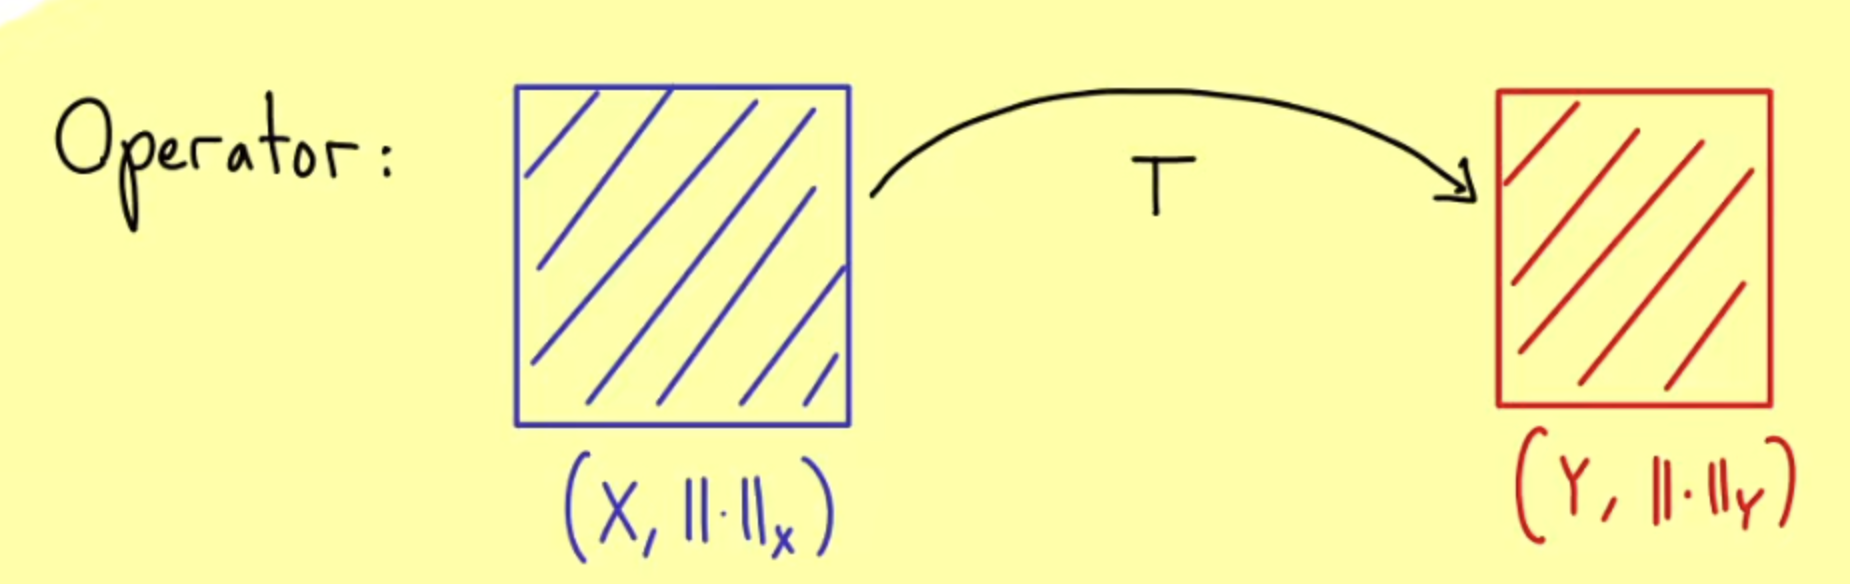
\includegraphics[scale = 0.4]{../figures/operator.png}
$T: X \rightarrow Y$, which satisfies
\begin{itemize}
    \item \textrm{linear (conserves the algebraic structure)}
    \item \textrm{continuous (bounded) (conserves the topological structure)}
\end{itemize}
\begin{definition}[Operator norm and bounded]
    $(X, \Vert \cdot \Vert_X)$, $(Y, \Vert \cdot \Vert)$ two normed spaces, $T: X \rightarrow Y$ linear, which means
    \begin{align}
        T(x+\tilde{x}) 
        &= T x + T \tilde{x} \\
        T(\lambda x)
        &= \lambda Tx
    \end{align}
    for all $x, \tilde{x} \in X$, $\lambda \in \mathbb{F}$. Then
    \begin{align}
        \Vert T \Vert 
        &= \Vert T \Vert_{X \rightarrow Y} \\
        &:= \sup\left\{\frac{\Vert Tx \Vert_Y}{\Vert x \Vert_X} \vert x \in X, x \neq 0 \right\}
    \end{align}
    is called the operator norm of $T$. If $\Vert T \Vert < \infty$, $T$ is called bounded.
\end{definition}
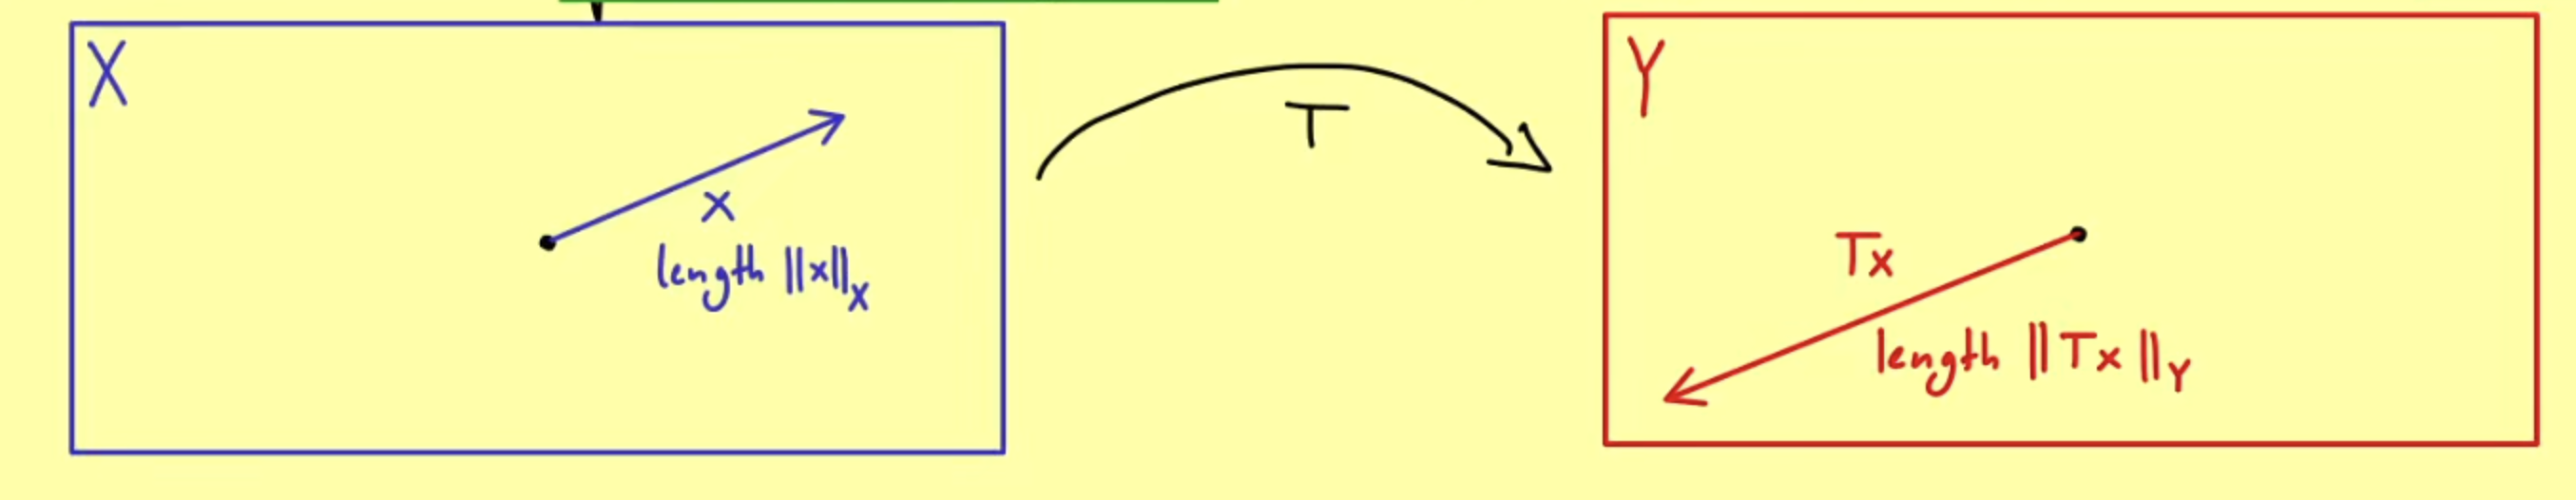
\includegraphics[scale = 0.3]{../figures/operator norm and bounded}

\begin{proposition}[Continuous equivalent to bounded]
    Let $(X, \Vert \cdot \Vert_X)$,$(Y, \Vert \cdot \Vert_Y)$ two normed spaces, $T: X \rightarrow Y$ linear. Then the following claims are equivalent:
    \begin{itemize}
        \item T~is~continuous.
        \item T~is~continuous~at~$x = 0$.
        \item T~is~bounded.
    \end{itemize}
\end{proposition}
\begin{proof}
    (a) $\Longrightarrow$ (b) is easily seen.

    (b) $\Longrightarrow$ (c): proposition (*): For all sequence $(x_n)_{n \in \mathbb{N}} \subseteq X$ with $x_n \stackrel{n \rightarrow \infty}{\longrightarrow} 0$, we have $T x_n \stackrel{n \rightarrow \infty}{\longrightarrow} 0$ due the properties of linear map.
    
    Claim: proposition (*) $\Longrightarrow$ proposition (+): there is a $\delta >0$ such that $\Vert Tx \Vert_Y <1$ for all $x \in X$ with $\Vert x \Vert_X < \delta$.

    proof of this claim: we prove its contraposition such that $\neg (*)$ $\Longrightarrow$ For all $n \in \mathbb{N}$, we find $x_n \in X$ with $\Vert x_n \Vert_X < \frac{1}{n}$ and $\Vert T x_n \Vert_Y \geq 1$ $\Longrightarrow$ $\neg (*)$.
    \begin{align}
        \frac{\Vert Tx \Vert_Y}{\Vert x \Vert_X}
        &= \frac{\Vert T x \Vert_Y \cdot \frac{\delta}{2}\cdot \frac{1}{\Vert x \Vert_X}}{\Vert x \Vert_X \cdot \frac{\delta}{2}\cdot \frac{1}{\Vert x \Vert_X}} \\
        &= \frac{\Vert T(\frac{\delta}{2}\frac{x}{\Vert x \Vert_X}) \Vert_Y}{\Vert \frac{\delta}{2} \frac{x}{\Vert x \Vert_X} \Vert_X} \\
        &\leq \frac{2}{\delta} \\
        &\Longrightarrow \Vert T \Vert = \sup\left\{\frac{\Vert Tx \Vert_Y}{\Vert x \Vert_X} \vert x \in X, x \neq 0 \right\} \leq \frac{2}{\delta}<\infty.
    \end{align}
    (c) $\Longrightarrow$ (a): Let $(x_n)_{n \in \mathbb{N}} \subseteq X$ be convergent with limit $\tilde{x} \in X$. Then $\Vert T x_n - T \tilde{x} \Vert_Y = \Vert T(x_n - \tilde{x}) \Vert_Y \leq \Vert T \Vert \cdot \Vert x_n - \tilde{x} \Vert_X \stackrel{n \rightarrow \infty}{\longrightarrow} 0$. 
\end{proof}
\SZQ{2023.04.02: This proof needs to be understood later.}

\SZQ{2023.04.02: Is should be proved that $\Vert T \Vert$ defined above is indeed a norm.}

\section{Part 14: Example Operator Norm}
\begin{example}
    $X = \left(C[0,1), \mathbb{F}, \Vert \cdot \Vert_{\infty}\right)$, $Y = \left(\mathbb{F}, \vert \cdot \vert \right)$. 
    For $g \in X$ with $g(t) \neq 0$ for all $t \in [0,1]$, define $T_g: X \rightarrow Y$ by $T_g(f):= \int_{0}^{1} g(t) \cdot f(t) {\rm d}t$. So what is $\Vert T_g \Vert$ ?
    \begin{proof}
    Recall that 
    \begin{align}
        \Vert F_g \Vert
        &= \sup\left\{\frac{\vert T_g(f) \vert}{\Vert f \Vert_{\infty}} \vert f \in X, f \neq 0 \right\} \\
        &\qquad\eqnote{This trick has been used before.} \nonumber \\
        &= \sup\left\{\frac{\vert T_g(f) \vert}{\Vert f \Vert_{\infty}} \vert f \in X, f \neq 0 \right\} \\
        &= \sup\left\{{\vert T_g(f) \vert} \vert f \in X, \Vert f \Vert_{\infty} = 1 \right\} \\
        &= \sup\left\{\vert \int_{0}^{1} g(t) \cdot f(t){\rm d}t \vert \vert f \in X, \Vert f \Vert_{\infty} = 1 \right\} \\
        &\qquad\eqnote{Since $\vert \int_{0}^{1}g(t)\cdot f(t){\rm d}t \vert \leq \int_{0}^{1}\vert g(t) \vert \cdot \vert f(t) \vert{\rm d}t $ and $\vert f(t) \vert \leq \Vert f \Vert_{\infty}=1$} \nonumber \\
        &\leq \int_{0}^{1} \vert g(t) \vert {\rm d}t \\
        &< \infty.
    \end{align}
    Check the other inequality: $h(t):= \frac{\overline{g(t)}}{\vert g(t) \vert}$ with $\Vert h \Vert_{\infty = 1}$. We then have
    \begin{align}
        \Vert T_g \Vert 
        &\geq \vert T_g(h) \vert \\
        &= \vert \int_{0}^{1} g(t) \frac{\overline{g(t)}}{\vert g(t) \vert} {\rm d}t \\
        &= \int_0^1 \frac{\vert g(t) \vert^2}{\vert g(t) \vert}{\rm d}t \\
        &= \int_0^1 \vert g(t) \vert{\rm d}t.
    \end{align}
    \end{proof}
\end{example}

\section{Part 16: Compact Sets}
\begin{example}
    Compactness $A \subseteq \mathbb{R}^n$. $A$ is compact such that 
    \begin{itemize}
        \item $A$ is closed. 
        \item $A$ is bounded.
    \end{itemize}
    This is only true in $\mathbb{R}^n$ or $\mathbb{C}^n$.
\end{example}
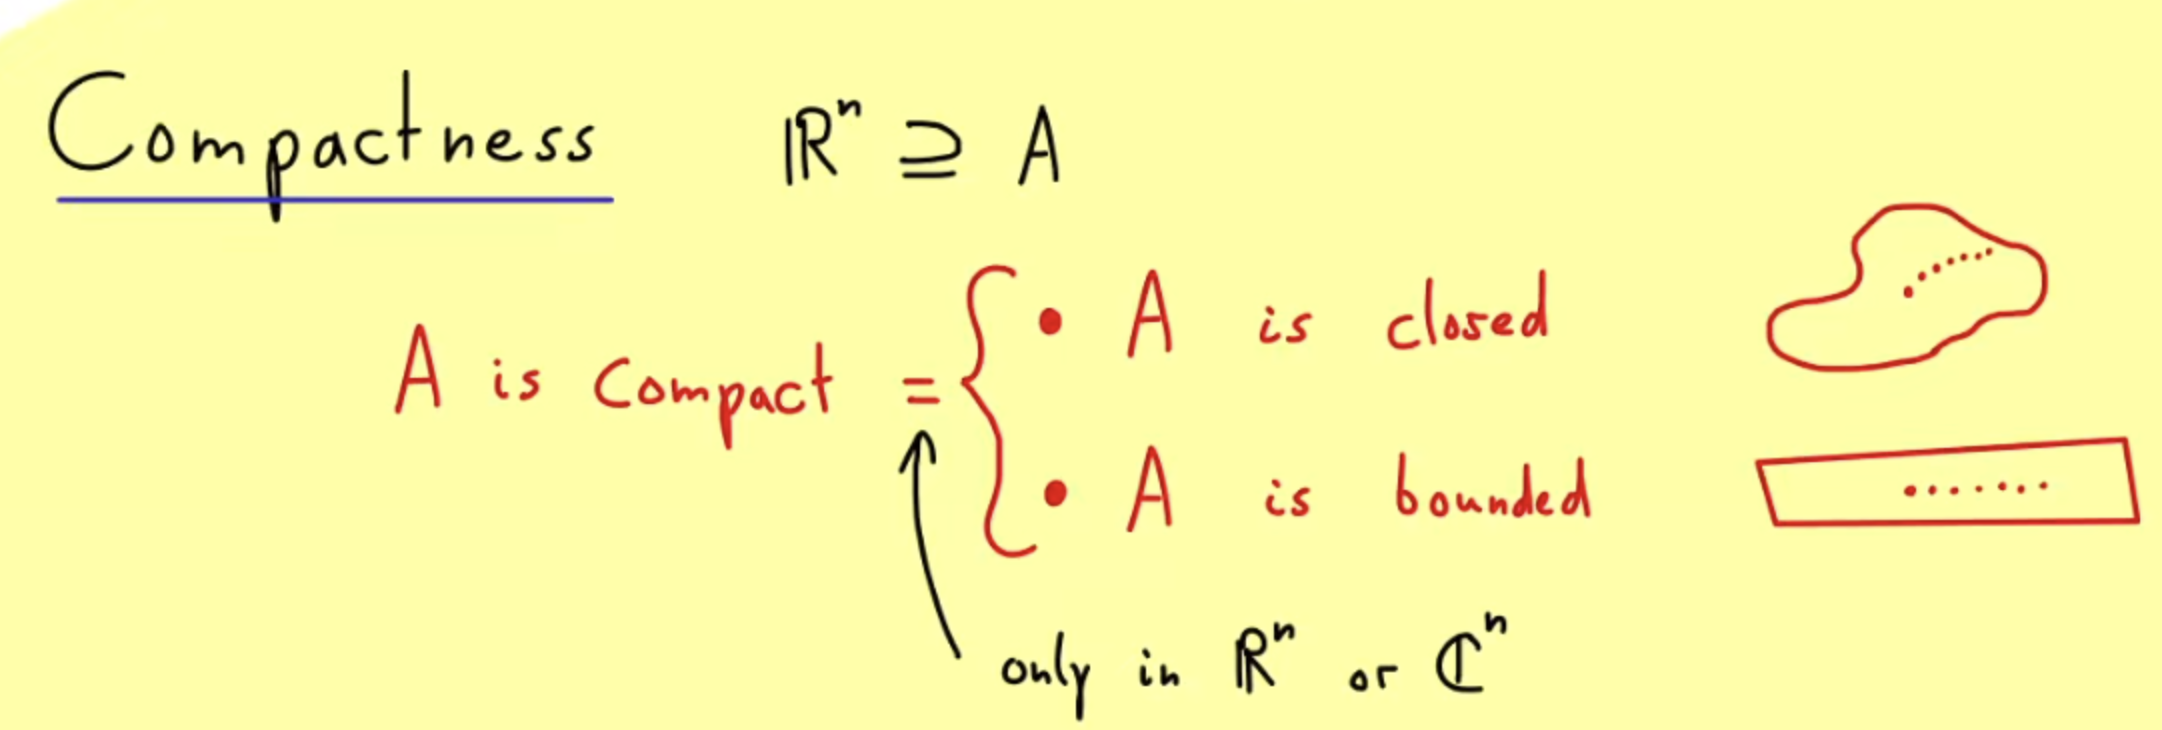
\includegraphics[scale = 0.3]{../figures/compactness.png}

\begin{definition}[Sequentially compact]
    Let $(X,d)$ be a metric space. $A \subseteq X$ is called (sequentially) compact if for each sequence $(x_n)_{n \in \mathbb{N}} \subseteq A$, one finds a convergent subsequence $(x_{n_k})_{k \in \mathbb{N}}$ with $\tilde{x}:= \lim_{k \rightarrow \infty} x_{n_k} \in A$.
\end{definition}
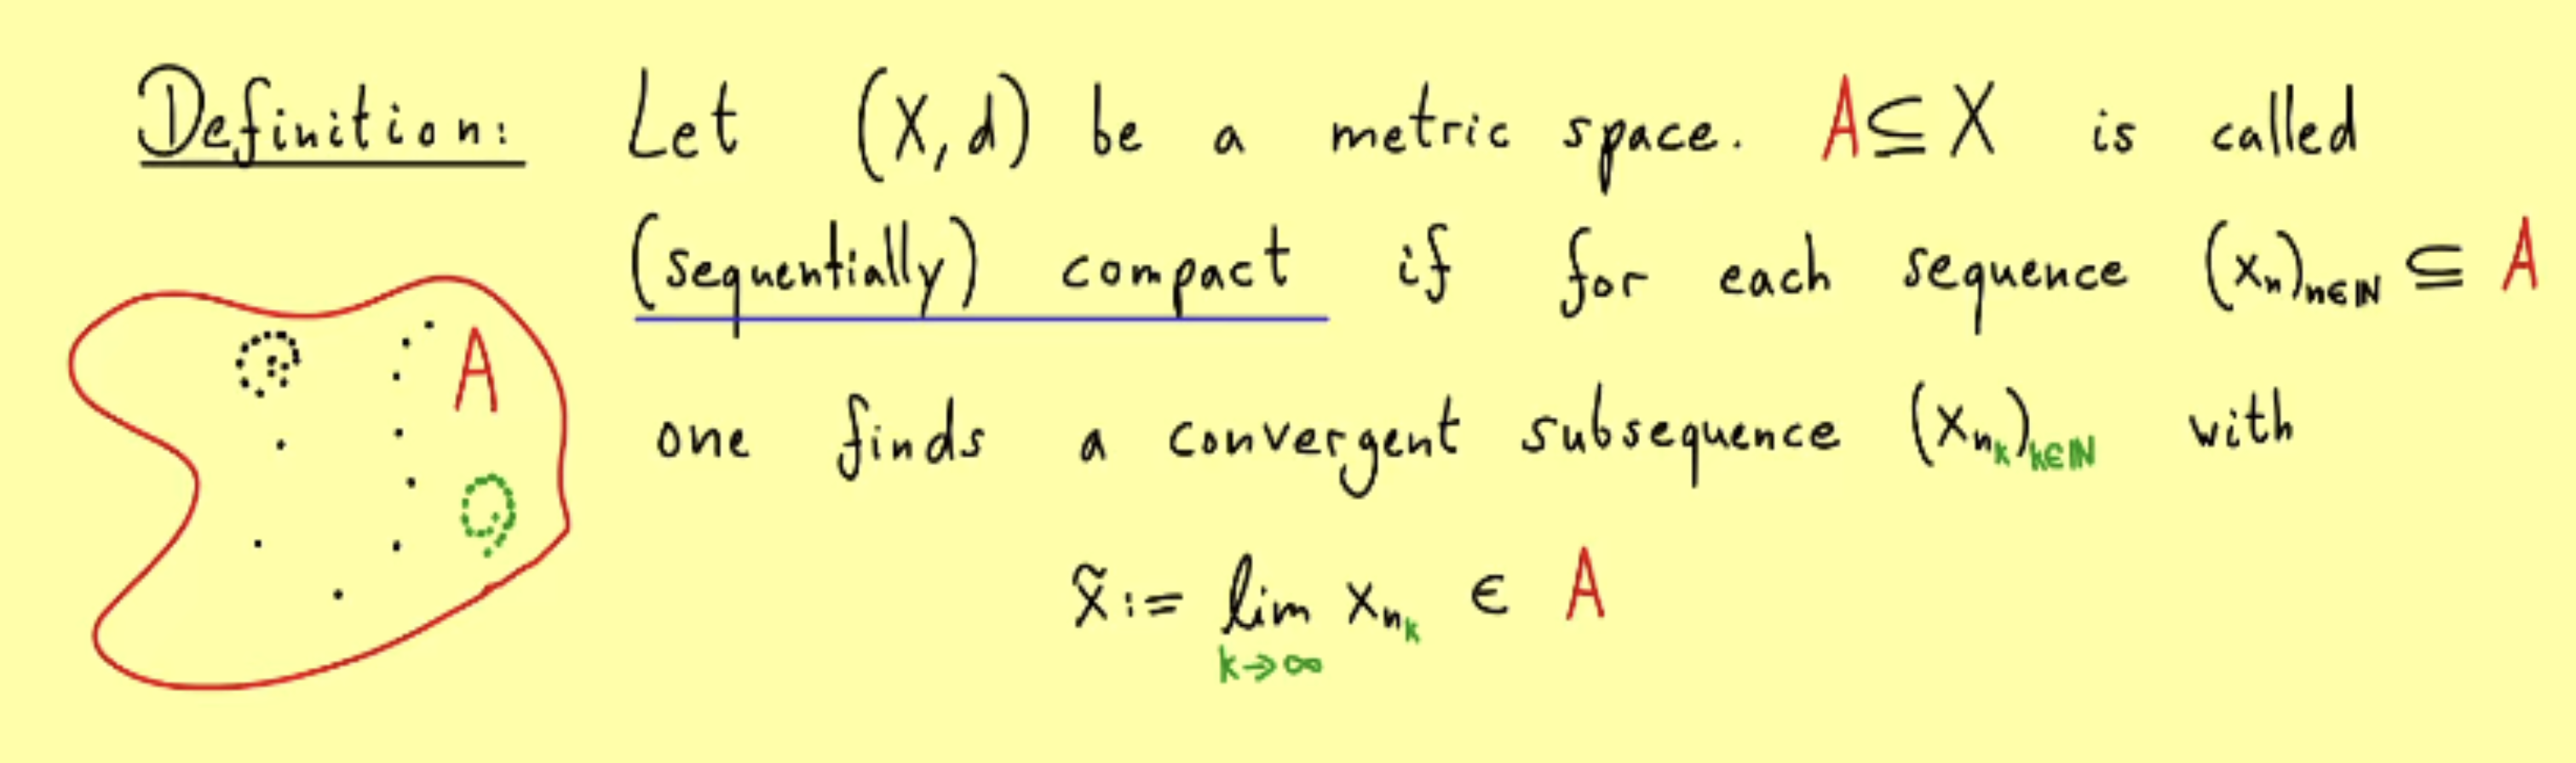
\includegraphics[scale = 0.2]{../figures/Sequentially compact.png}

\begin{example}
    \begin{itemize}
        \item $(\mathbb{R},d_{eucl.})$, $A = [0,1]$ compact by Bolzano-Weierstrass theorem.
        \item $(\mathbb{R}, d_{discr})$, $A=[0,1]$ not compact because: The sequence $(x_n)_{n \in \mathbb{N}} \subseteq A$ with $x_n =\frac{1}{n}$ satisfies $d_{discr.}(x_n,x_m)=1$ for all $n,m \in \mathbb{N}$ with $n \neq m$. $\Longrightarrow$ no convergent subsequence.  
    \end{itemize}
\end{example}
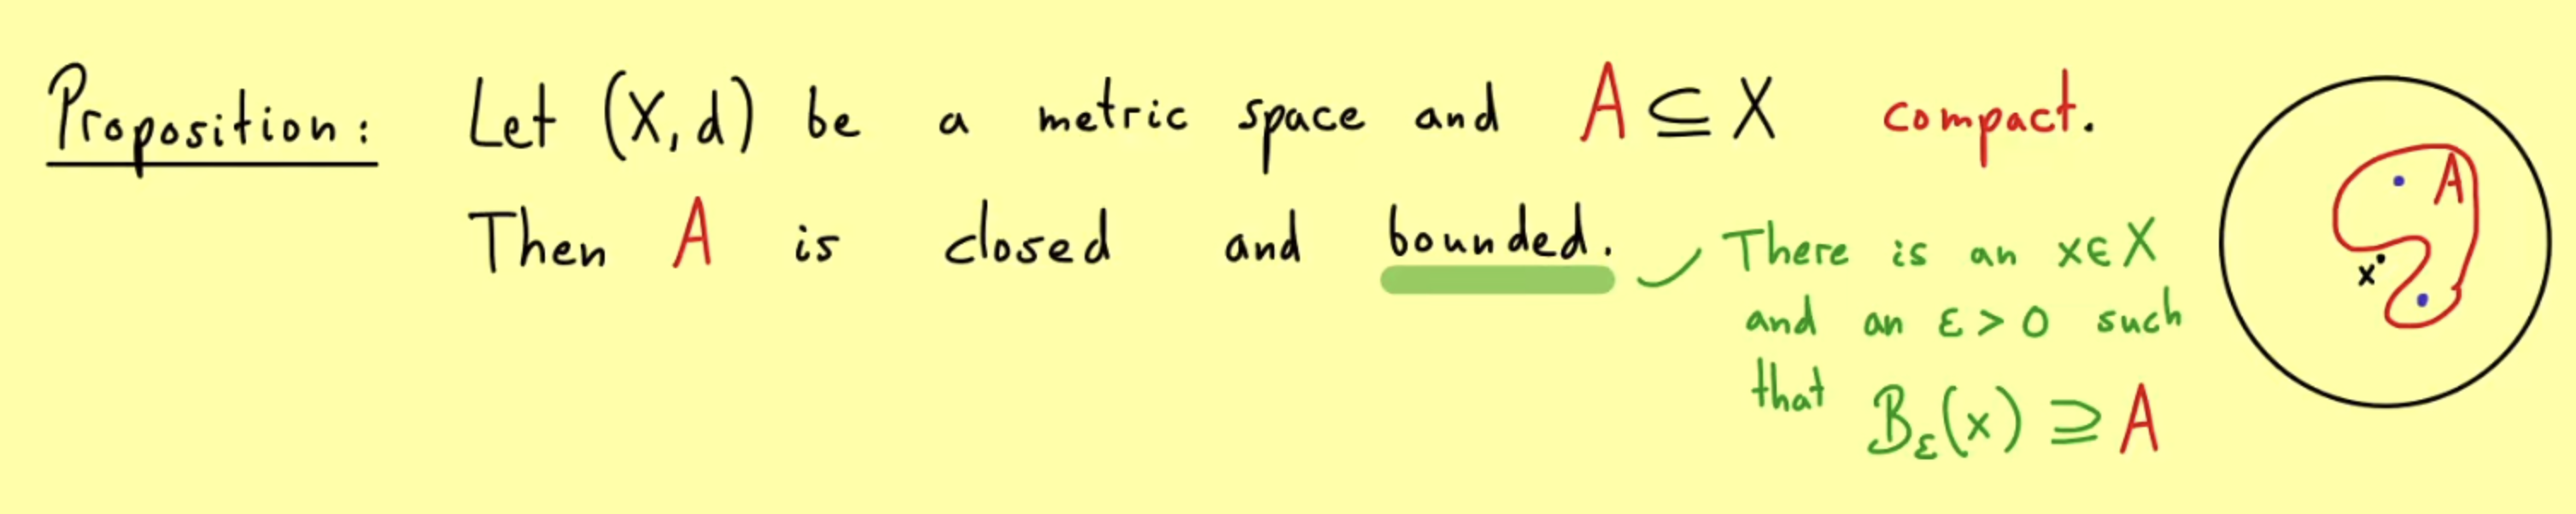
\includegraphics[scale = 0.2]{../figures/def of bounded.png}
\begin{definition}[Bounded]
    Let $(X,d)$ be a metrix space and $A \subseteq X$ compact. $A$ is bounded means that there is an $x \in X$ and an $\varepsilon > 0$ such that $A \subseteq B_{\varepsilon}(x)$.
\end{definition}
\begin{proposition}[Compact implies closed and bounded]
    Let $(X,d)$ be a metrix space and $A \subseteq X$ compact. Then $A$ is closed and bounded.
\end{proposition}
\begin{proof}
    Let $A \subseteq X$ be compact.

    (1) Let $(x_n)_{n \in \mathbb{N}} \subseteq A$ be convergent with limit $\tilde{x} \in X$. 
    \begin{align}
        &\Longrightarrow \textrm{There is aa convergent subsequence}~(x_{n_k})_{k \in \mathbb{N}}~\textrm{with limit}~\tilde{\tilde{x}} \in A \\
        &\Longrightarrow \tilde{x} = \tilde{\tilde{x}} \in A \\
        &\Longrightarrow A~is~closed!
    \end{align}  

    (2) contraposition: $A$ is not bounded.

    $\Longrightarrow$ For given $a \in A$, there are $x_n \in A$ with $d(a,x_n)>n$.

    $\Longrightarrow$ For any subsequence $(x_{n_k})_{k \in \mathbb{N}}$ and any point $b \in A$:
    \begin{align}
        n_K
        &< d(a,x_{n_k}) \\
        &\leq d(a,b) + d(b,x_{n_k})
    \end{align}

    $\Longrightarrow$ $n_k - d(a,b)\leq d(b, x_{n_k})$.

    $\Longrightarrow$ $d(b,x_{n_k}) \stackrel{k \rightarrow \infty}{\longrightarrow} 0$ for all $b \in A$

    $\Longrightarrow$ $A$ not compact!
\end{proof}

\section{Part 18: Compact operators}
\begin{definition}[Compact operators]
    Let $(X, \Vert \cdot \Vert_X)$, $(Y, \Vert \cdot \Vert_Y)$ be two normed spaces. A bounded linear operator $T: X \rightarrow Y$ is called compact if $\overline{T[B_1(0)]} \subseteq Y$ is a compact set.
\end{definition}
\SZQ{2023.04.02: the defintion of $\overline{T[B_1(0)]} \subseteq Y$ should be learned first.}

\section{Part 19: Holder's inequality}
\begin{lemma}[Young's inequality]
    \label{lemma: Young's inequality}
    For all $a,b > 0 $, we have $a,b\leq \frac{a^p}{p} + \frac{b^{p^\prime}}{p^\prime}$.
\end{lemma}
\begin{proof}
    Note that function $f: x \mapsto e^x$ is convex, we have
    \begin{align}
        f(\lambda x + (1-\lambda) y )
        &\leq \lambda f(x) + (1-\lambda) f(y).
    \end{align}
    Let $\lambda = \frac{1}{p}$, $x = \ln a^p $, $1-\lambda = \frac{1}{p^\prime}$, and $y = \ln b^{p^\prime}$. We have
    \begin{align}
        a \cdot b = f(\frac{1}{p}  \ln a^p + \frac{1}{p^\prime} \ln b^{p^\prime} ) = f(\lambda x + (1-\lambda) y )
        &\leq \lambda f(x) + (1-\lambda) f(y) \\
        &=\frac{1}{p} f(\ln a^p) + \frac{1}{p^\prime} f(\ln b^{p^\prime}) \\
        &= \frac{a^p}{p} + \frac{b^\prime}{p^\prime}.
    \end{align}
\end{proof}

\begin{theorem}[Holder's inequality]
    \label{lemma: Holder's inequality}
    For all $x,y \in \mathbb{F}^n$, we have 
    \begin{align}
        \Vert xy \Vert_1 \leq \Vert x \Vert_p \cdot \Vert y \Vert_{p^\prime},
    \end{align}
    where $x \in \mathbb{F}^n$ and the p-norm of x is
    \begin{align}
        \Vert x \Vert_q
        &:= \left(\sum_{j=1}^{n} \vert x_j \vert^q \right)^{\frac{1}{q}},
    \end{align}
    $q \in [1,\infty)$, $\frac{1}{p} + \frac{1}{p^\prime} = 1$, and for $x,y \in \mathbb{F}^n$, we write
    \begin{align}
        xy
        &:= \left(\begin{matrix}
            x_1 y_1 \\
            x_2 y_2 \\
            ... \\
            x_n y_n
        \end{matrix}\right).
    \end{align}
\end{theorem}
\begin{proof}
    Case 1: $x = 0$ or $y = 0$.

    Case 2: We have
    \begin{align}
        \frac{1}{\Vert x \Vert_p \Vert y \Vert_{p^\prime}} \Vert xy \Vert_1 
        &= \frac{1}{\Vert x \Vert_p \Vert y \Vert_{p^\prime}} \sum_{j=1}^n \vert x_j y_j \vert \\
        &= \sum_{j=1}^n \frac{\vert x_j \vert}{\Vert x \Vert_p} \frac{\vert y_j \vert}{\Vert y \Vert_{p^\prime}} \\
        &\qquad\eqnote{By Young's lemma (\ref{lemma: Young's inequality})} \nonumber \\
        &\leq \sum_{j=1}^n \frac{1}{p} \cdot \frac{\vert x_j \vert^p}{\Vert x \Vert^p_p} +  \sum_{j=1}^n \frac{1}{p^\prime} \cdot \frac{\vert y_j \vert^{p^\prime}}{\Vert x \Vert^{p^\prime}_{p^\prime}} \\
        &=\frac{1}{p} + \frac{1}{p^\prime} \\
        &= 1.
    \end{align}
\end{proof}

\section{Part 21: Isomorphism?}
\begin{definition}[Homomorphism]
    \textbf{What is Homomorphism: map that preserves structures.}
\end{definition}
\SZQ{When we talk about homophism, we must know the underlying structures!}

\begin{example}
    \begin{itemize}
        \item Let $X,Y$ be vector spaces and $f: X \rightarrow Y$ be a map. We want
        \begin{align}
            f(\lambda \cdot x)
            &= \lambda \cdot f(x) \\
            f(x+x')
            &= f(x) + f(x'),
        \end{align}
        which is called linear. Thus homomorphism = linear map!
        \item Let $(X,d_X), (Y,d_Y)$ be two metric spaces and $f: X \rightarrow Y$ be a map. We want 
        \begin{align}
            d_Y(f(x),f(x'))\leq d_X(x,x').
            \label{eq: homo for metric space}
        \end{align}
        homomorphism = map that satisfies (\ref{eq: homo for metric space})
    \end{itemize}
\end{example}
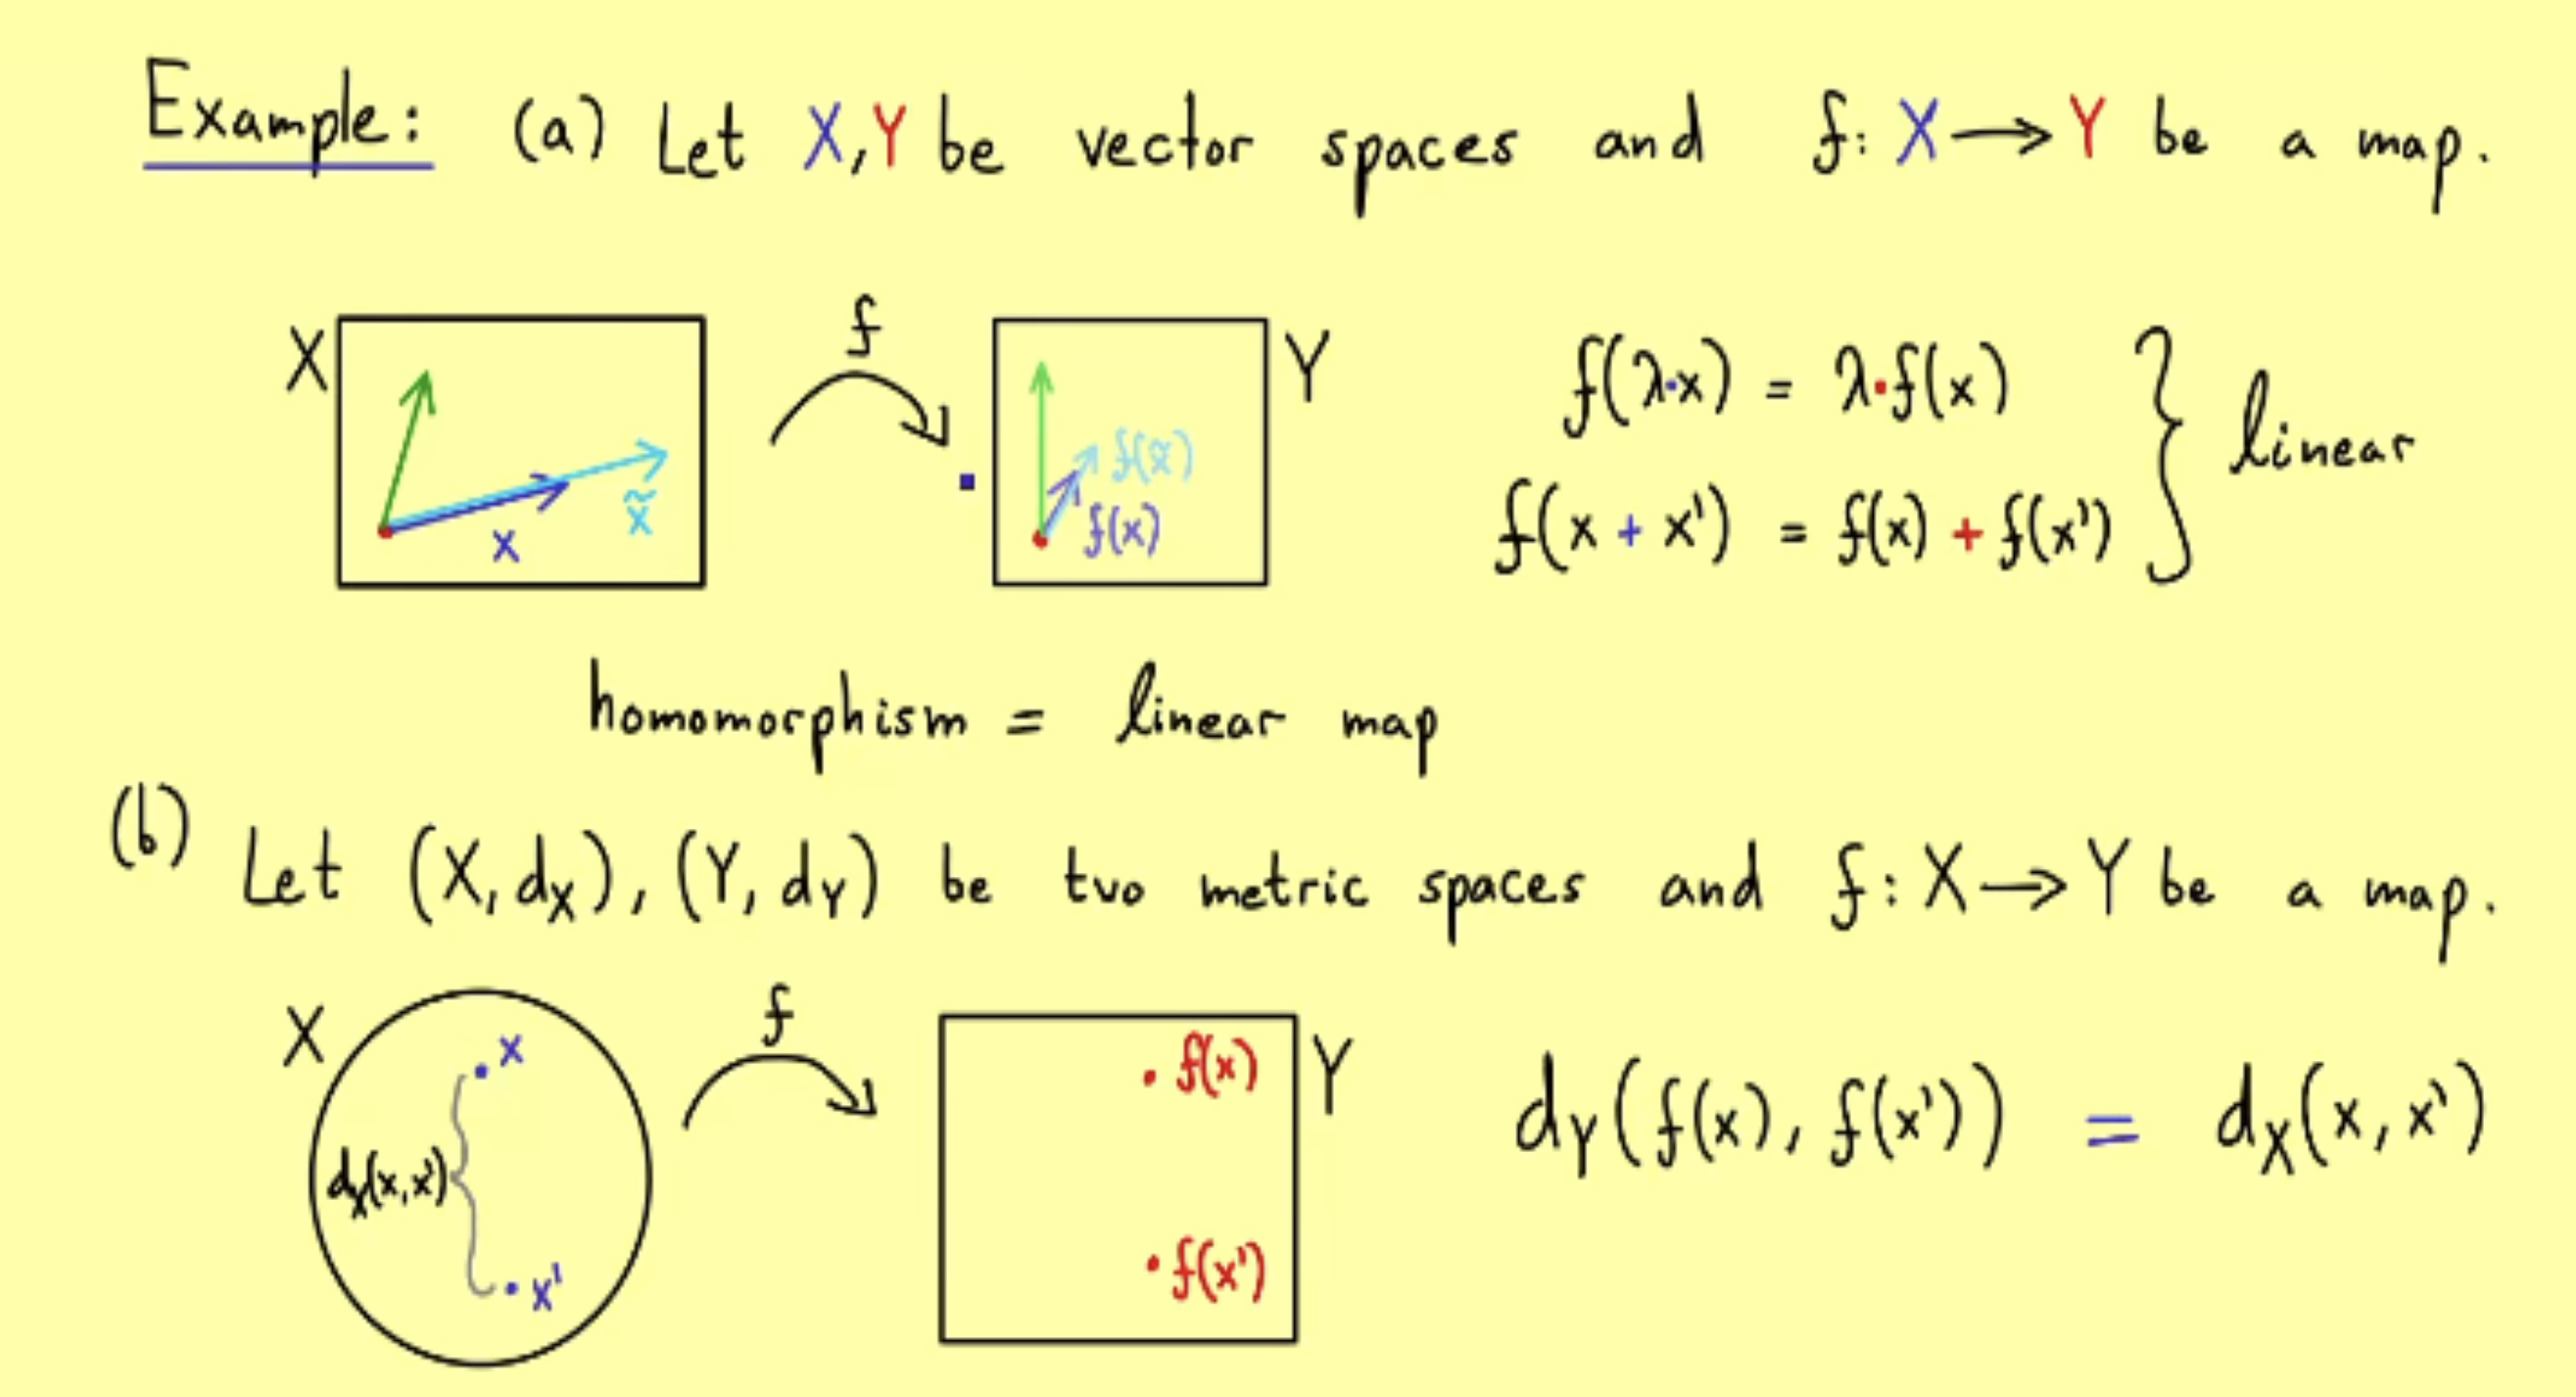
\includegraphics[scale = 0.25]{../figures/homomorphism.png}

\begin{definition}[Isomorphism]
    Isomorphism = homomorphism + bijective + inverse map is also homomorphism
\end{definition}

\begin{definition}[Isomorphism for Banach spaces]
    Isomorphism for banach spaces $X,Y$: $f: X \rightarrow Y$ with: linear + bijective + $\Vert f(x) \Vert_Y = \Vert x \Vert_X$ (oftern called isometric isomorphism).
\end{definition}

\begin{example}
    \begin{itemize}
        \item $S_R: l^p(\mathbb{N}) \rightarrow l^p(\mathbb{N})$, $(x_1, x_2,x_3,\dots) \mapsto (0,x_1,x_2,\dots)$ 
        \begin{align}
            &\Longrightarrow \textrm{linear, $\Vert S_R x \Vert_p = \Vert x \Vert_p$ not surjective} \\
            &\Longrightarrow \textrm{not an isomorphism}
        \end{align}
        \item $S: l^p(\mathbb{Z}) \rightarrow l^p(\mathbb{Z})$, $(\dots, x_{-1}, x_0,x_1,\dots) \mapsto (\dots,x_{-2},x_{-1}, x_0, \dots)$ 
        \begin{align}
            &\Longrightarrow \textrm{linear, $\Vert S x \Vert_p = \Vert x \Vert_p$ and bijective} \\
            &\Longrightarrow \textrm{isomorphism}
        \end{align}
    \end{itemize}
\end{example}

\section{Part 22: Dual spaces}
\begin{proposition}
    Let $X$ be a normed space. Then $(X', \Vert \cdot \Vert_{X \rightarrow \mathbb{F}})$ is a Banach space.
\end{proposition}
\begin{proof}
    
\end{proof}

\SZQ{2023.04.02: I need to learn Riesz representation theorem!}
\section{Part 28: Spectrum for bounded linear operators}
Recall: $A \in \mathbb{C}^{n \times n}$ matrix with $n$ rows and $n$ columns. $\lambda \in \mathbb{C}$ is called an eigenvalue of $A$ if:
\begin{align}
    &\exists x \in \mathbb{C}^n \backslash \left\{0\right\}: Ax = \lambda x \\
    &\Longleftrightarrow \exists x \in \mathbb{C}^n \backslash \left\{0\right\}: (A - \lambda I) x = 0 \\
    &\Longleftrightarrow {\rm Ker}(A - \lambda I) \neq \left\{0\right\} \\
    &\Longleftrightarrow map~x \mapsto (A-\lambda I)x~not~injective.
\end{align}

\begin{theorem}[Rank-nullity theorem]
    For any matrix $M \in \mathbb{C}^{m \times n}$:
    \begin{align}
        dim(Ran(M)) + dim(Ker(M)) = n.
    \end{align}
\end{theorem}

\begin{definition}[Spectrum and resolvent]
    Let $X$ be a complex Banach space and $T: X \rightarrow X$ be a bounded linear operator. Then the spectrum of $T$ is defined by:
    \begin{align}
        \sigma(T)
        &:= \left\{\lambda \in \mathbb{C} \vert (T - \lambda I) not~bijective\right\}.
    \end{align}
    The resolvent of $T$ is defined by:
    \begin{align}
        \rho(T)
        &:= \left\{\lambda \in \mathbb{C} \vert (T - \lambda I) ~bijective~and~(T - \lambda I)^{-1}~bounded \right\}.
    \end{align}
\end{definition}

\begin{corollary}
    By bounded inverse theorem, we have
    \begin{align}
        \sigma(T)
        &= \mathbb{C} \backslash \rho(T).
    \end{align}
\end{corollary}

\begin{definition}[Point/continuous/residual spectrum]
    We have the disjoint union: $\sigma(T) = \sigma_{p}(T) \cup \sigma_{c}(T) \cup \sigma_r(T)$. We have
    \begin{align}
        \textrm{Point spectrum}:
        &\sigma_{p}:= \left\{\lambda \in \mathbb{C} \vert (T- \lambda I)~not~injective\right\}, \\
        \textrm{Continuous spectrum}:
        &\sigma_{c}:= \{\lambda \in \mathbb{C} \vert \\
        &(T- \lambda I)~injective~but~not~surjective~with~\overline{Ran(T-\lambda I)} = X \}, \\
        \textrm{Residual spectrum}:
        &\sigma_{r}:= \{\lambda \in \mathbb{C} \vert \\
        &(T- \lambda I)~injective~but~not~surjective~with~\overline{Ran(T-\lambda I)} \neq X \}. \\
    \end{align}
\end{definition}

\SZQ{2023.04.02: I need to learn injective, surjective, bijective first!}

\section{Part 31: Spectral Radius}
\begin{definition}[Spectral radius]
    $X$ complex Banach space. $T: X \rightarrow X$ bounded lineara operator. We define the spectral radius as
    \begin{align}
        r(T)
        &:= \sup\left\{\vert \lambda \vert \right\},
    \end{align}
    where $\lambda \in \sigma(T)$.
\end{definition}
Here, we have a fig to show this def.

\begin{theorem}
    $X$ complex Banach space, $T: X \rightarrow X$ bounded linear operator. Then 
    \begin{itemize}
        \item $\sigma(T) \subseteq \mathbb{C}$ is compact
        \item $X\neq\left\{0\right\}$ $\Longrightarrow$ $\sigma(T)\neq \emptyset$
        \item $r(T):= \sup \vert \lambda \vert = \lim_{k \rightarrow \infty} \Vert T^k \Vert^{\frac{1}{k}} = \inf_{k \rightarrow \mathbb{N}} \Vert T^k \Vert^{\frac{1}{k}} \leq \Vert T \Vert < \infty$,
    \end{itemize}
    where $\lambda \in \sigma(T)$
\end{theorem}
\begin{proof}
    
\end{proof}

\SZQ{2023.04.02: I need to learn the properties of sepctrum, dual spaces, Vom-Neuman series, Liouville's theorem, Hahn-Banach Theorem!}

\section{Part 32: Normal and Self-Adjoint Operators}
\begin{definition}[Adjoint operator]
    Let $X$ be a Hilbert space and $T: X \rightarrow X$ a bounded lineaar operator. The bounded linear operator $T^\ast: X \rightarrow X$ defined by
    \begin{align}
        \langle y, Tx \rangle
        &= \langle T^\ast y, x \rangle, \forall x,y \in X
    \end{align}
    is called the adjoint operator of $T$.
\end{definition}

\begin{definition}[Self Adjoint operator]
    Let $X$ be a Hilbert space and $T: X \rightarrow X$ a bounded lineaar operator. $T$ is called 
    \begin{itemize}
        \item self-adjoint if $T^\ast = T$ 
        \item skew-adjoint if $T^\ast = -T$
        \item normal if $T^\ast T = T T^\ast$
    \end{itemize}
\end{definition}

\begin{proposition}
    T is normal $\Longrightarrow$ $r(T) = \Vert T \Vert$.
\end{proposition}


\end{document}